
\subsection{Human Computer Interfaces for Assistive Robotics} 
%\sububsection{Overview}
There is a long history of assistive robotic systems using electrophysiological signals as input, with work going back as far as  \cite{schmidl-65} and \cite{sherman-65}. In the time since, there have been myriad approaches and refinements of proposed of interfaces for disabled individuals with robotic assistive systems, and this work will not review even a small fraction of them. There are two ways of categorizing these systems. One way is to categorize a system by its input modality; i.e. whether it uses physical buttons or pointing devices, some external sensor of motion such as eye or hand trackers, or some specific electrophysiological signal such as EMG, electrooculagraphy (EOG), and EEG.  Within this category, modalities can be further divided by where the signals are recorded from. EMG can be recorded from distal muscle sites, which may be larger, easier to record from, and produce larger signals. However, more impaired individuals tend to maintain control over muscle functions closer to the head

Another way to categorize the systems is by the type of control they engender - whether the control is at a task level, allowing the user to designate what is to be done, or at a state level, allowing the user to specify joint angles, or end effector positions.  

This work presents a system at an intermediate control level, in which the user has some state level control that is task oriented. This requires an online planning system that generates robust grasps in real-time. Below we describe the different control paradigms used in related systems using human-robot interface (HRI) devices suitable for impaired individuals.  

\subsubsection{Direct Demonstration}
 The most intuitive, low level of control of a robotic arm involves having the robot arm directly mimic the motions of the user. It is possible to reconstruct a user's movements using distal limb surface EMG signals, as in \cite{Artemiadis2011,Castellini2009}.  This type of control allows the user to express their desires explicitly, allowing the user to specify how the arm is to avoid obstacles. This paradigm is not suitable for assistive robotic interfaces because many seriously impaired individuals have lost exactly the capability used as the control input to this type of interface.  
 
 \subsubsection{Joint Level Control}
If direct mimicry is impractical, the user can be given explicit control of joints of the robot. This generally imposes a much higher cognitive load on the user, as they have to attend closely to each joint. The movement of the joints are not directly related to user's goal of manipulating some object. Control of a manipulator through such an interface is generally not possible because they have many joints. The manipulator is generally controlled by simple open and close commands. For example, in \cite{Horki2011} hand opening/closing and elbow flexion/extension are controlled by EEG signals.

 For a prosthetic arm with essentially two degrees of freedom, this sort of control may be appropriate, but more degrees of freedom will strain the bit rate of these types of devices and their unreliability will make the coordination necessary to perform complex tasks in natural environments difficult or impossible. For example, to grasp an object using a six DOF manipulator with a gripper, the user must move in a straight line towards an object, or the gripper will not move straight and the finger may knock over the object while moving the palm into place.  This requires that the user simultaneously send coordinated signals to all six degrees in exactly the right ratios, or it may not move in anything close to a straight line.  

\subsubsection{End Effector Cartesian Control}
The main goal of a robotic manipulator is to interact with the world with some end effector. Giving the user direct control over the end effector location can be more intuitive, because the end effector location is the variable that the user most directly observes. This control scheme has been implemented using both invasive high throughput systems as in  \cite{Vogel2010},  and less invasive systems with lower throughput such as surface facial EMG and EOG, as in \cite{Postelnicu2011, Sagawa2005,Gomez-Gil2011,Ranky2010,Shenoy2008}.  Although this approach is similar to joint level control in requiring continuous attention to a relatively large number of degrees of freedom simultaneously, the user's control is directly in the task space. This allows the user to decouple the different controlled degrees of freedom.   

\subsubsection{Discrete State Level Control}
In discrete mode control, the user is able to switch between a set of predetermined configurations. This control paradigm is commonly used for control of robotic hands to swithc between a number of different hand configurations, as in \cite{Yang2009a,Woczowski2010,Ho2011,Cipriani2008,Matrone2011}.

 These control schemes represent a tradeoff between flexibility and simplicity of use. This tradeoff is especially important for as the complexity of the hand increases. Direct control over the fingers of a complex manipulator is not feasible because of the number of DOFs and the precision required to avoid collisions. Discrete level control allows more DOFs to be controlled safely with fewer inputs.

However, these schemes limit the user's flexibility to the preset configurations. Additionally, the user has to remember how to get to the configuration that they want to use at a given time, which may require multiple steps through a branching decision tree.  Because there is not necessarily an easy way of associating the path that they need to take in that decision tree with the goal they want to reach, these control schemes have a steep learning curve. 

\subsubsection{Task Level Control}
The key challenge of using noninvasive human robot interfaces is that the bit rate is low and that the input is somewhat unreliable. In addition, the user experiences limited feedback, which makes direct control difficult.  Under these conditions, it would seem intuitive that users would find task level control, where the user directs the robot on what to do but has little input as to how to, would be more effective. Indeed,  it has been shown that users find HRI control easier using even higher level, goal oriented paradigms \cite{Royer2011}, and we have begun to see work that attempts to exploit higher level abstractions to allow users to perform more complex tasks with robotic arms. 

In \cite{Bell2008}, EEG signals were used to select targets for pick and place operations for a small humanoid robot. \cite{Waytowich} used EEG signals to control pick and place operations of a 4-DOF St\"{a}ubli robot. \cite{M.BryanV.ThomasG.NicollL.Chang2011} presented preliminary work extending this approach to a grasping pipeline on the PR2 robot. In that work, a 3D perception pipeline is used to find and identify target objects for grasping and EEG signals are used to choose between them. In \cite{Muller-Putz2005}, grasping is decomposed to a four-phase pipeline where EEG signals are used to control transitions between phases. And in \cite{Scherer2011a}, the authors demonstrate an interface to navigate in two dimensions and select goals in a complex virtual environment and propose a hierarchical control scheme for learning high-level tasks dynamically. 

The drawback of this approach is that while the system presents the user with a set of high level choices, the user is not able to effect the process by which the choices are generated. In complex situations, the software agent may not present the user with appropriate choices. 

\subsubsection{Task Oriented Shared Control}
An emerging alternative to the purely task oriented approach is to blend end effector control and task oriented control. In this approach, the user's input demonstrates some approximation of the desired solution or constraint which an automated planner can make use of. \cite{Mulling2015} showed that this strategy can improve performance in grasping tasks even when using an invasive BCI device with relatively high bandwidth. In our work, we show that this strategy can allow non-invasive devices with much lower bandwidth to exercise similar performance in accomplishing complex tasks with high reliability. 

\subsection{The Eigengrasp Grasp Planner}
 In Ciocarlie et al. [2009], our lab introduced the Eigengrasp Planner, which allowed the user to grasp objects reliably by demonstrating only an approximate approach direction. In this work, we have expanded upon the Eigengrasp planner to show that task oriented shared control is a practical approach for allowing the flexibility of lower level control schemes with the ease of use of higher level task level control. 

\begin{figure}[b]
	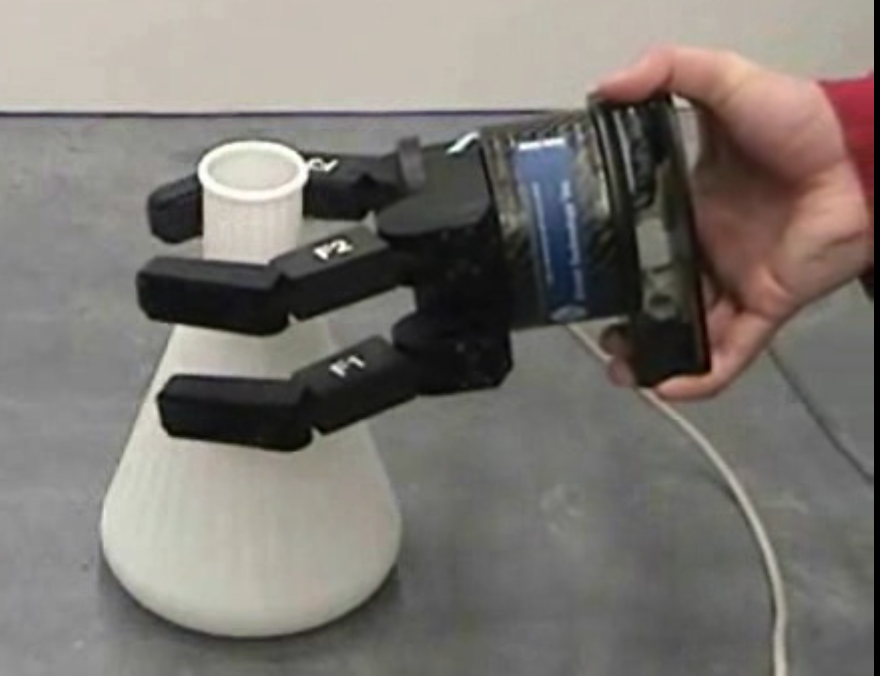
\includegraphics[height=2in]{images_2/real_eg_grasp.png}
	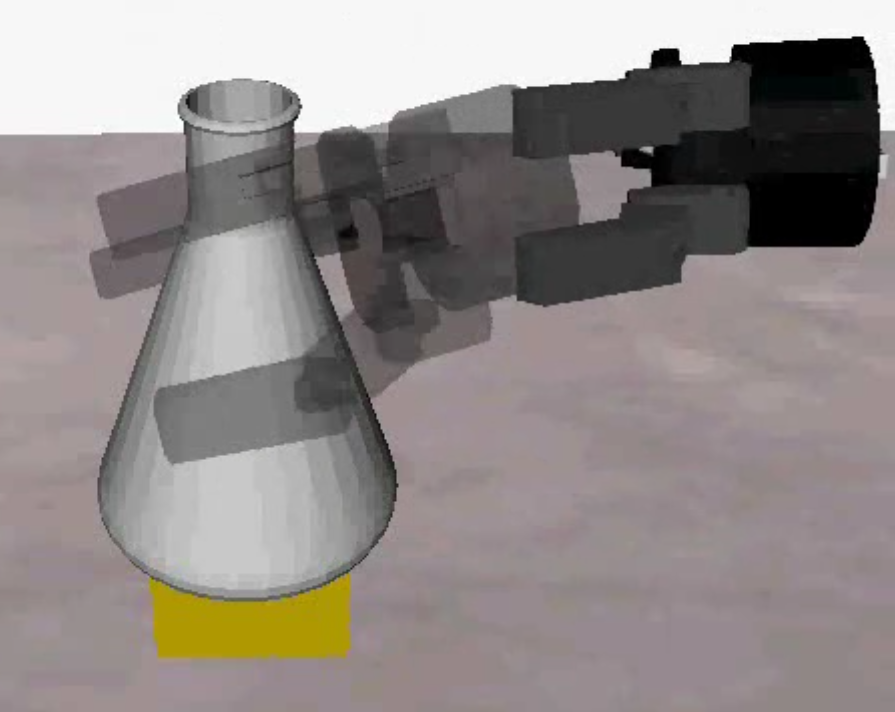
\includegraphics[height=2in]{images_2/simulated_eg_grasp2.png}
	\caption{An operator demonstrating the Eigengrasp Planner by manually guiding the robotic hand to guide the planner in the virtual environment.\cite{CiocarlieIJRR}}
	\label{fig:egplanner_demo} 
\end{figure}

The Eigengrasp Planner allows a user to interact with an online grasp planner in a virtual environment to plan grasps online in real-time. The user is given control of a virtual representation of the hand which they use to indicate approximately where they would like to grasp the object. A grasp planner runs in the background and presents the user with a set of options for completing the grasp. 
This strategy requires a responsive planner that can handle the complex problem of grasp planning in near real-time. To make this computationally tractable, Eigengrasps were introduced, a dimensionality reduction technique in which control of the hand is mapped to principle components identified in human grasping studies. With this dimensionality reduction, stochastic sampling techniques can be used to generate reasonably good grasps in real-time using relatively simple grasp quality metrics.
 
The quality metric that is used by the planner evaluates a projection of the desired contact points on the hand to the target object. This projection provides a smooth energy gradient in regions where the hand is not in contact with the object. When good candidates are found, the planner simulates completing the grasp by approaching the object along a pre-specified direction orthogonal to the "palm" of the robot hand and then closing the fingers. 

This approach has a number of practical advantages. The nature of the optimization approach, which gradually moves towards lower values of the quality function, produces solutions where nearby finger contacts will also provide similar quality grasps. Grasps where the qualities of nearby configurations are much poorer will have narrow basins of attraction that are less likely to be found. This implies a certain amount of robustness to small displacements and occlusion of the object from nearby clutter during grasp acquisition. The planner is easy to generalize because the only robot specific parameters are the state space reduction strategy and a set of desirable contact locations, which can be easily specified for any given robot. 

In Ciocarlie et al. [2009], the planner was demonstrated by having the operator manually move the end effector in real-time (see Figure \ref{fig:egplanner_demo}). This is analogous to an extremely high bandwidth, low noise interface with perfect knowledge of the environment. In this work, we have fleshed out this demonstration to more realistic, complex situations. This required development of a full robotic grasping platform that can handle cluttered scenes, realistic input devices appropriate for disabled people, and an augmented reality user interface. The development of such a system is the central challenge addressed in this paper.  


\subsection{ Roadmap of this paper}

To address this challenge, we have iterated through four designs of our assistive robotics system, denoted System 1-4. Section III presents an initial prototype, named \emph{System 1}, tested on a single user and first reported in \cite{Weisz2012c}, which we very briefly summarize.  Section IV describes user experiments using \emph{System 2}, which improves on the prototype system with additional UI elements that allow more flexible and effective user control. In Section V, we describe \emph{System 3} which integrates the novel EMG interface device and allows grasping in cluttered scenes, and test its efficacy with an impaired user. In Section VI, we describe \emph{System 4} which improves the speed and reliability of the user interface and demonstrates it on a cohort of healthy subjects. 


















